\subsection{Asignatura}

  \paragraph{}Se procede a crear las asignaturas a las se matricula el alumno,
  en este caso, las mencionadas en el capítulo \ref{enunciado},
  \textit{Enunciado}. Para ello, se realizará la creación de las asignaturas,
  tal y como se describió en el capítulo \ref{addAsignatura},
  \textit{Añadir asignatura}.

  \paragraph{}Una vez que aparezca el formulario de creación, se debe introducir
  el nombre de cada asignatura, con lo que la pantalla quedaría tal y como
  refleja la figura \ref{ejemploAddAsignatura} para el caso de la asignatura
  \textit{Biología molecular}. El resto de asignaturas siguen el mismo proceso
  de creación, con sus respectivos detalles.

  \begin{figure}[!ht]
    \begin{center}
      \fbox{
      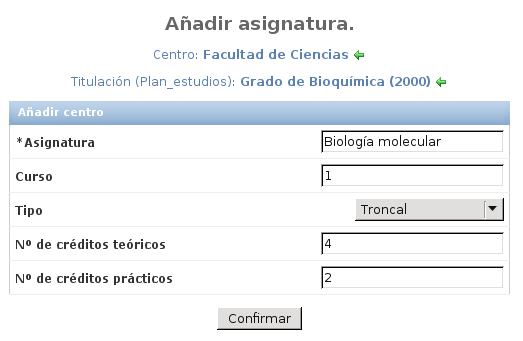
\includegraphics[scale=0.55]{5.Ejemplos_Practicos/5.3.IntroduccionDatos/5.3.3.Asignatura/add_asignatura.png}
      }
      \caption{Creación de \textit{Asignatura} de ejemplo.}
      \label{ejemploAddAsignatura}
    \end{center}
  \end{figure}

  \paragraph{}Una vez rellenado el formulario, se pulsará el botón
  \textit{Confirmar}, el cual se puede ver en la figura
  \ref{capturaBotonConfirmar}. Si el formulario rellenado es válido, y no tiene
  errores, se creará el nuevo elemento en el sistema. En caso de contener
  información no válida, un mensaje de error aparecerá indicando los campos
  del formulario que no han pasado la validación, los cuales habrá que modificar
  para introducir correctamente el elemento en el sistema.
